\documentclass[11pt,reqno]{amsart}
\usepackage{graphicx}
\usepackage{enumerate}
\usepackage{mathtools}
\usepackage[margin=1in]{geometry}
\usepackage{booktabs}
\usepackage{graphicx}
\usepackage{amsmath}
\usepackage{hyperref}
\usepackage{subcaption} % 导入 subcaption 包以支持子图
\usepackage{float}
\renewcommand{\theequation}{\arabic{enumi}.\arabic{equation}}

\DeclareMathOperator{\im}{im}
\DeclareMathOperator{\rank}{rank}
\DeclareMathOperator{\nullity}{nullity}
\DeclareMathOperator{\tr}{tr}

\newcommand{\tp}{{\scriptscriptstyle\mathsf{T}}}
\usepackage{listings} 
\usepackage{xcolor} 
\lstset{
  language=C++,                 % 设置语言为 C++
  basicstyle=\ttfamily,          % 使用等宽字体
  keywordstyle=\color{blue},     % 关键字高亮为蓝色
  commentstyle=\color{green},    % 注释高亮为绿色
  stringstyle=\color{red},       % 字符串高亮为红色
  numberstyle=\tiny\color{gray}, % 行号高亮为灰色
  numbers=left,                  % 行号显示在左侧
  stepnumber=1,                  % 每行显示行号
  frame=single,                  % 给代码加一个边框
  breaklines=true,               % 自动换行
  backgroundcolor=\color{lightgray!20}, % 设置背景颜色
  captionpos=b,                  % 标题在底部
  showspaces=false,              % 显示空格
  showstringspaces=false,        % 在字符串中显示空格
}
\lstdefinestyle{python}{
    language=Python,
    basicstyle=\ttfamily\small,  % Code font size
    keywordstyle=\bfseries\color{blue},
    commentstyle=\itshape\color{green!50!black},
    stringstyle=\color{orange},
    showstringspaces=false,
    frame=single,                % Adds a border around the code
    numbers=left,                % Line numbers on the left
    numberstyle=\tiny\color{gray},
    breaklines=true,             % Automatic line breaking
    captionpos=b,                % Caption at the bottom
    tabsize=4,                   % Tab size
}
\setlength{\parindent}{0pt}
\begin{document}
\title[]{Project2:Ensemble data assimilation with ML model\\Chu Zhuyiheng 12455799}
\maketitle


\section{Ensemble data assimilation with ML model}

The script \verb|test_addCRPS.py| has completed the task.

The following three figures show the results of the filtering performance comparison when the mean observation error is 0.1. The numerical ensemble size is set to 5, and the ML ensemble sizes are set to 20, 50, and 200, respectively. 

From the figures, it can be observed that the filtering effect corresponding to the numerical ensemble is significantly better. Interestingly, a larger ML ensemble size leads to increased error, contrary to my expectations.

\begin{figure}[h]
  \centering
  % Subfigure 1: ML Ensemble Size = 20
  \begin{subfigure}[t]{0.65\textwidth}
      \centering
      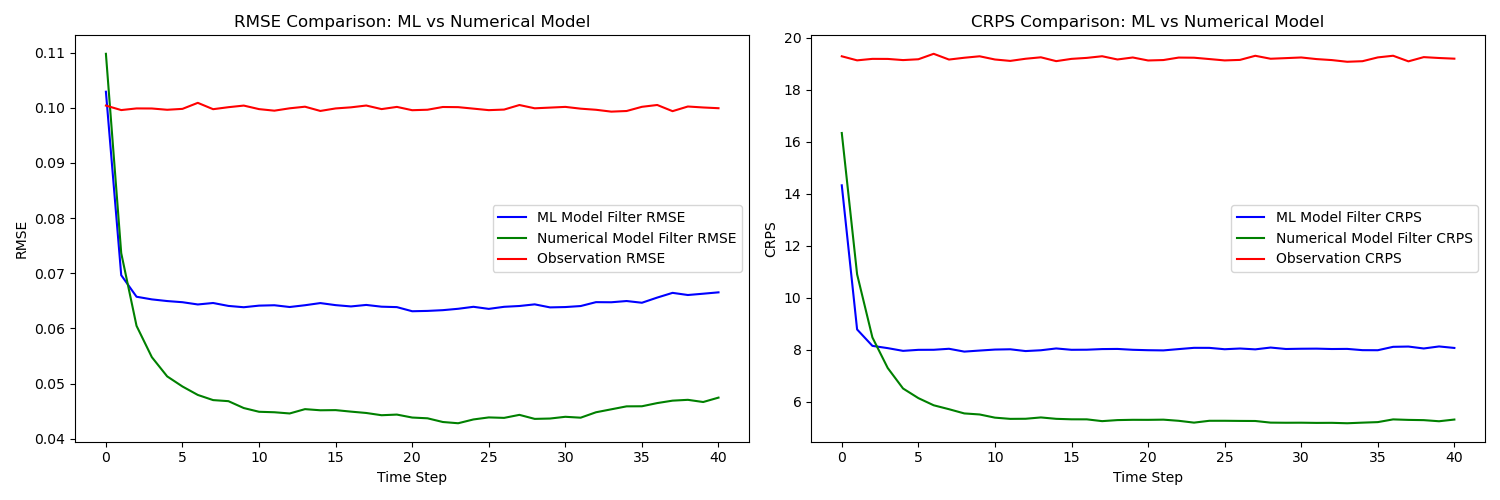
\includegraphics[width=\textwidth]{/mnt/c/workspace/study/Inverse Problem and Data Assimilation/project/Project2/pic/n40_sz5&20_r4_num&ml_noise0.1.png} % Replace with actual image file
      \caption{ML Ensemble Size = 20.}
      \label{fig:ml-ensemble-20}
  \end{subfigure}
  \vspace{0.5cm}
  
  % Subfigure 2: ML Ensemble Size = 50
  \begin{subfigure}[t]{0.65\textwidth}
      \centering
      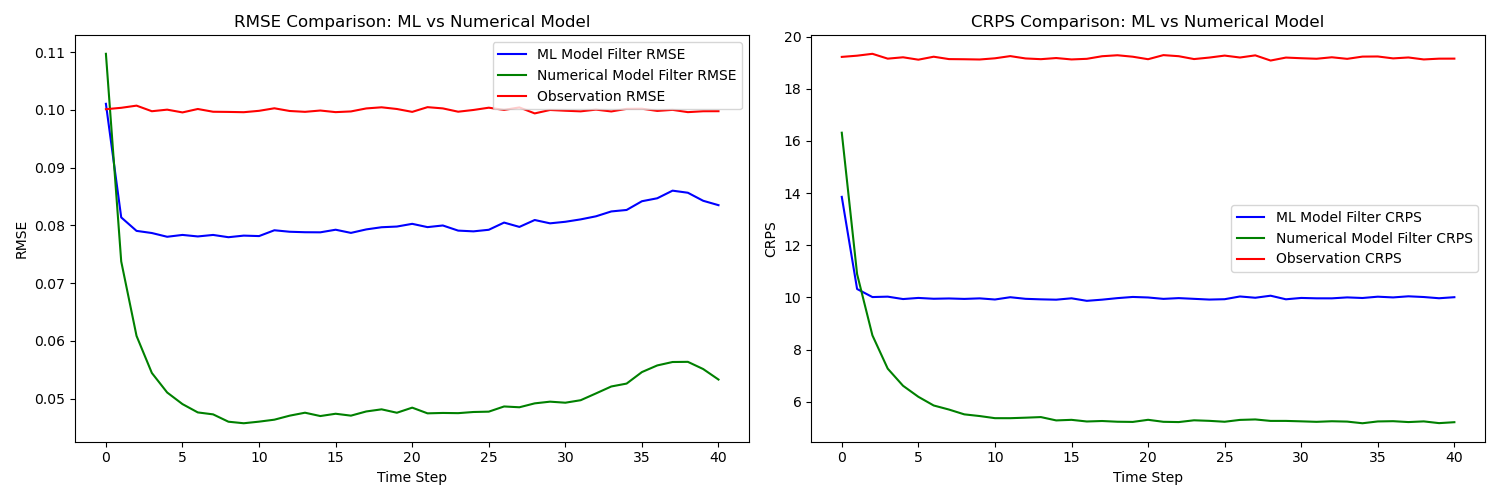
\includegraphics[width=\textwidth]{/mnt/c/workspace/study/Inverse Problem and Data Assimilation/project/Project2/pic/n40_sz5&50_r4_num&ml_noise0.1.png} % Replace with actual image file
      \caption{ML Ensemble Size = 50.}
      \label{fig:ml-ensemble-50}
  \end{subfigure}
  \vspace{0.5cm}
  
  % Subfigure 3: ML Ensemble Size = 200
  \begin{subfigure}[t]{0.65\textwidth}
      \centering
      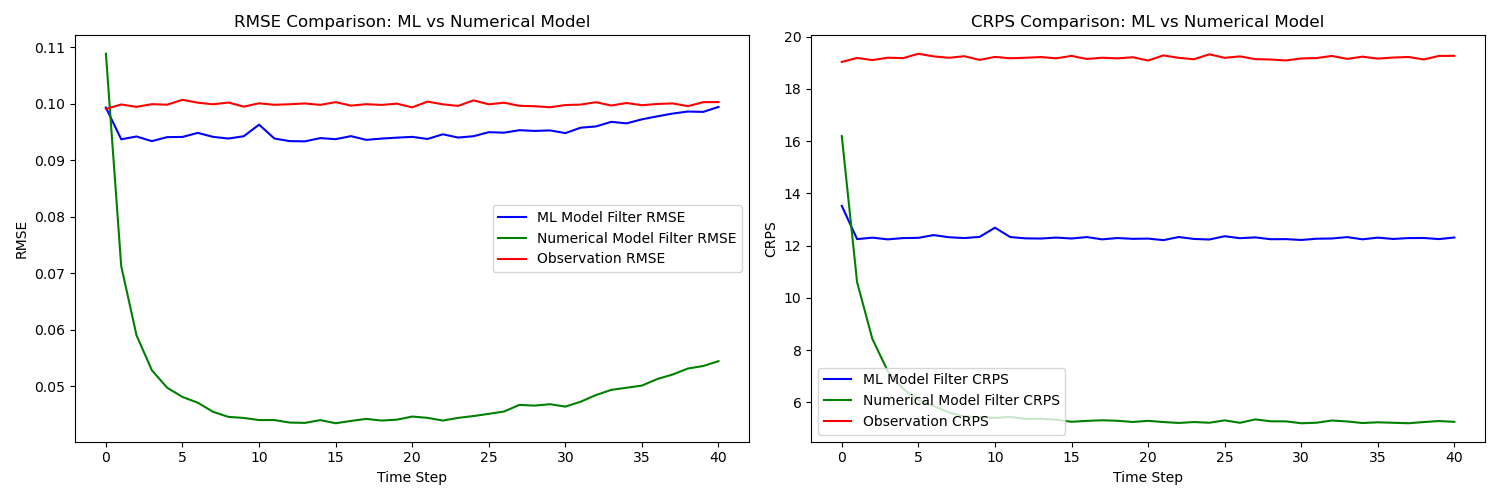
\includegraphics[width=\textwidth]{/mnt/c/workspace/study/Inverse Problem and Data Assimilation/project/Project2/pic/n40_sz5&200_r4_num&ml_noise0.1.png} % Replace with actual image file
      \caption{ML Ensemble Size = 200.}
      \label{fig:ml-ensemble-200}
  \end{subfigure}

  \caption{Comparison of filtering performance with numerical ensemble size = 5 and ML ensemble sizes = 20, 50, and 200.}
  \label{fig:ensemble-comparison}
\end{figure}

However, the ensemble size cannot be too small. The following figure shows the results when the ensemble size is 2 and 10 respectively. It can be found that the error becomes larger than the observation error, which is obviously unacceptable.

\begin{figure}[htbp]
  \centering
      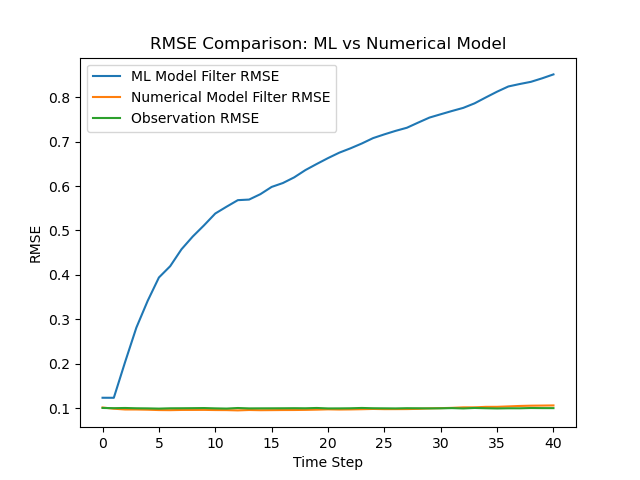
\includegraphics[width=\textwidth]{/mnt/c/workspace/study/Inverse Problem and Data Assimilation/project/Project2/pic/n40_sz2&10_r4_num&ml_noise0.1.png} % Replace with actual image file
      \caption{Numberical Ensemble Size = 2. ML Ensemble Size = 10. Get a big error}
      \label{fig:ensemble-size-2}
\end{figure}

\section{Attempts at cut-off radius and localization methods}

The previous section basically covers the content required to achieve Project goals. Next, I will talk about the problems I encountered when doing the project and the solutions.

The problem is that the dimension of the problem state is too large. The covariance matrix that needs to be constructed is about 30k*30k size. The computer memory is insufficient and the running time is very long.

A paper~\cite{houtekamer_1998} I found pointed out that it is possible to set a cutoff radius and simply ignore the covariances beyond this radius.
This method can make the covariance matrix sparse, solving the problems of insufficient memory and long running time.

I tried this method but it didn't work well.
\begin{figure}[H]
  \centering
      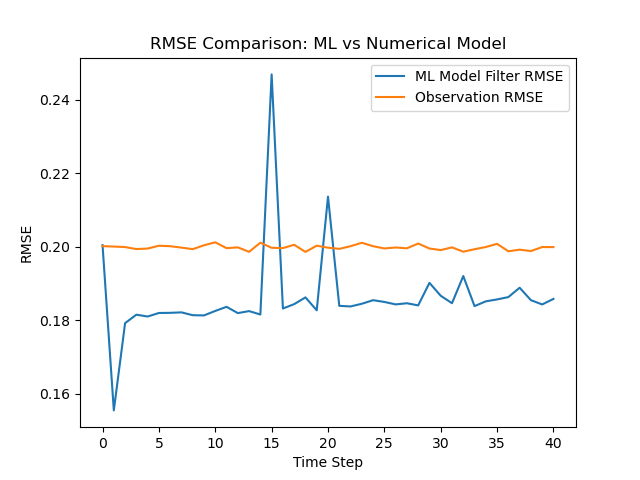
\includegraphics[width=0.5\textwidth]{/mnt/c/workspace/study/Inverse Problem and Data Assimilation/project/Project2/pic/n40_sz100_r2_newlocal.png} % Replace with actual image file
      \caption{Cutoff radius = 2}
\end{figure}

Then I found another article~\cite{houtekamer_2001} by the same author, which mentioned that the Schur product can be used instead of the cutoff radius method. This article uses a very complex compact support function for the Schur product. For the sake of convenience, I directly use the linear function of the distance.

\begin{figure}[H]
  \centering
      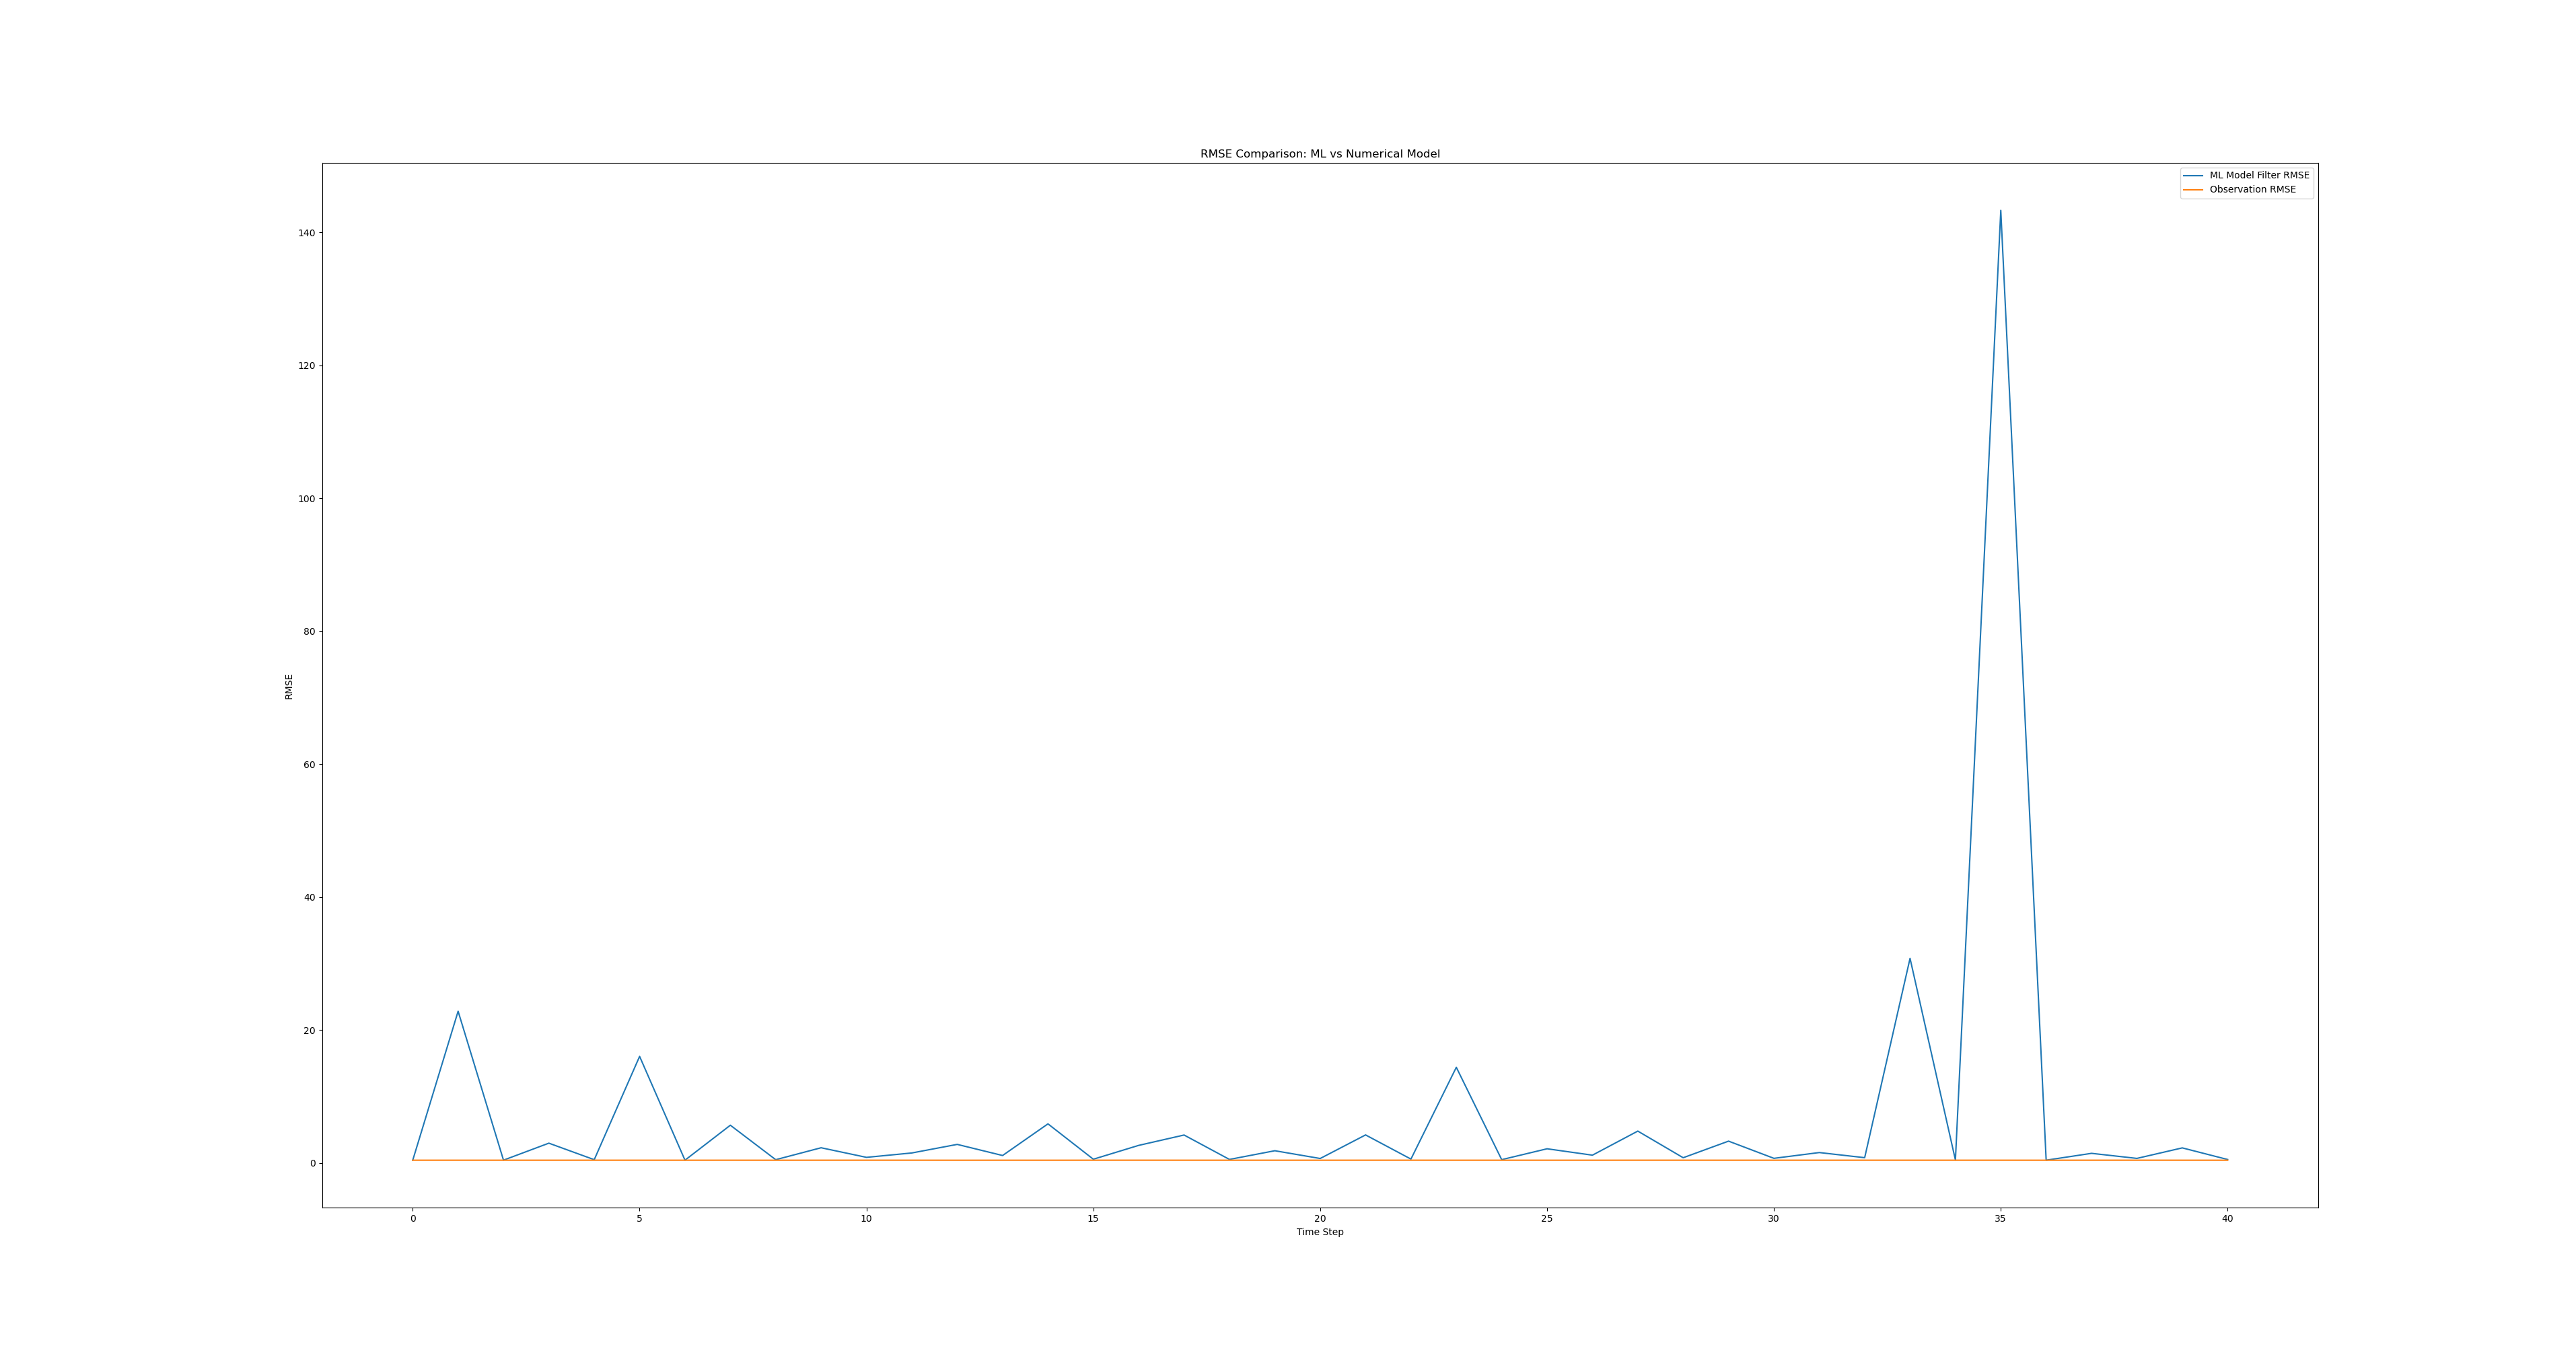
\includegraphics[width=\textwidth]{/mnt/c/workspace/study/Inverse Problem and Data Assimilation/project/Project2/pic/n40_sz200_r2.png} % Replace with actual image file
      \caption{Cutoff radius = 2, Schur product method for localization}
\end{figure}

It can be found that the effect is very poor, but the article mentions that for the same set size, the error will first decrease and then increase as the cutoff radius increases.

Then I tried increasing the cutoff radius and got the following results:

\begin{figure}[H] % Floating environment (ensure subcaptions are inside this)
  % Second Row
  \begin{subfigure}[h]{0.45\textwidth}
      \centering
      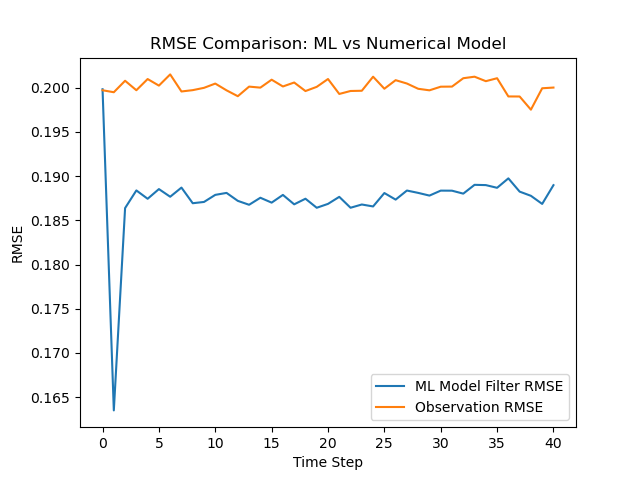
\includegraphics[width=\textwidth]{/mnt/c/workspace/study/Inverse Problem and Data Assimilation/project/Project2/pic/n40_sz200_r3.png} % Replace with actual image file
  \caption{Cutoff radius = 3, Schur product method for localization}
  \end{subfigure}
  \hfill
  \begin{subfigure}[h]{0.45\textwidth}
      \centering
      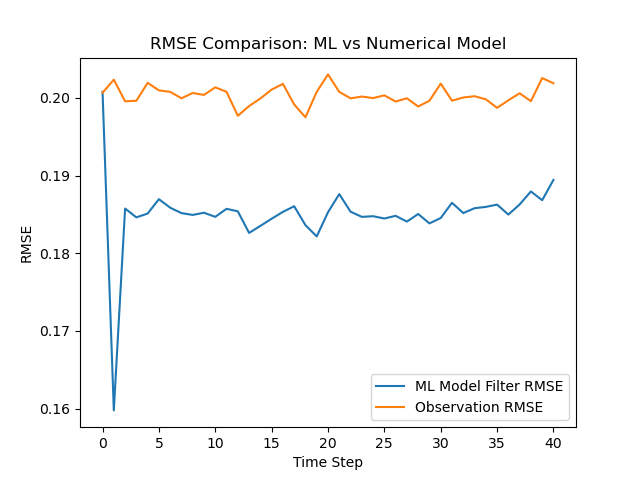
\includegraphics[width=\textwidth]{/mnt/c/workspace/study/Inverse Problem and Data Assimilation/project/Project2/pic/n40_sz200_r4.png} % Replace with actual image file
  \caption{Cutoff radius = 4, Schur product method for localization}
  \end{subfigure}
\end{figure}
It can be found that the error has been significantly improved. The results corresponding to the larger cutoff radius cannot be run due to insufficient computer performance.

The results in the previous section are obtained by running ENKF based on the optimal parameters here. (cutoff radius is 4, using Schur product method for localization)
\begin{thebibliography}{9}
  \bibitem{houtekamer_1998}
  Houtekamer, P. L. and Mitchell, H. L. (1998). 
  Data Assimilation Using an Ensemble Kalman Filter Technique. 
  \textit{Monthly Weather Review}, \textit{126}(3), 796--811. 
  \href{https://journals.ametsoc.org/view/journals/mwre/126/3/1520-0493_1998_126_0796_dauaek_2.0.co_2.xml}{link}.
  \bibitem{houtekamer_2001}
  Houtekamer, P. L. and Mitchell, H. L. (2001). 
  A Sequential Ensemble Kalman Filter for Atmospheric Data Assimilation. 
  \textit{Monthly Weather Review}, \textit{129}(1), 123--137. 
  \href{https://journals.ametsoc.org/view/journals/mwre/129/1/1520-0493_2001_129_0123_asekff_2.0.co_2.xml}{link}.
    
\end{thebibliography}
  
\end{document}